\documentclass[14pt]{article}

\usepackage[utf8x]{inputenc}
\usepackage[russian]{babel}
\usepackage{graphicx}
\graphicspath{{images/}}
\DeclareGraphicsExtensions{.pdf,.png,.jpg}

\usepackage{amsmath}
\usepackage{pgfplots}

\usepackage{geometry} % Меняем поля страницы
\geometry{left=2cm}% левое поле
\geometry{right=1.5cm}% правое поле
\geometry{top=2cm}% верхнее поле
\geometry{bottom=2cm}% нижнее поле

\renewcommand{\theenumi}{\arabic{enumi}}% Меняем везде перечисления на цифра.цифра
\renewcommand{\labelenumi}{\arabic{enumi}}% Меняем везде перечисления на цифра.цифра
\renewcommand{\theenumii}{.\arabic{enumii}}% Меняем везде перечисления на цифра.цифра
\renewcommand{\labelenumii}{\arabic{enumi}.\arabic{enumii}.}% Меняем везде перечисления на цифра.цифра
\renewcommand{\theenumiii}{.\arabic{enumiii}}% Меняем везде перечисления на цифра.цифра
\renewcommand{\labelenumiii}{\arabic{enumi}.\arabic{enumii}.\arabic{enumiii}.}% Меняем везде перечисления на цифра.цифра

\begin{document}
\begin{titlepage}
	\begin{center}
		\fontsize{18pt}{20pt}\selectfont
		\textbf{Работа 1.4.5.}	
	
		\vspace{5cm}
		\fontsize{24pt}{25pt}\selectfont
		Экспериментальная проверка закона вращательного движения на крестообразном маятнике
	\end{center}
	\begin{flushright}
		\fontsize{18pt}{20pt}\selectfont
		\vspace{14cm}
		\hspace{-3cm}
		\textit{Корнеев Е.С.}
	\end{flushright}		
\end{titlepage}

\begin{center}
	\fontsize{16pt}{18pt}\selectfont	
	Экспериментальная проверка закона вращательного движения на крестообразном маятнике
\end{center}

\fontsize{14pt}{16pt}\selectfont
\vspace{1cm}
Основное уравнение вращательного движения тела вокруг закреплённой оси:

\begin{equation}
I\varphi'' = M
\end{equation}

\vspace{1cm}
\textbf{Цель работы:} экспериментально проверить уравнение (1), получив зависимость углового ускорения от момента инерции и момента прикладываемых к системе сил, а также проанализировать влияние сил трения, действующих в оси вращения. \textbf{Экспериментальная установка.} Для экспериментального исследования закона вращательного движения (1) в работе используется крестообразный «маятник», устройство которого изображено на рис. 1. Маятник состоит из четырех тонких стержней радиуса $a$, укрепленных на втулке под прямым углом друг к другу. Втулка и два шкива различных радиусов ($r_1$ и $r_2$) насажены на общую ось. Ось закреплена в подшипниках, так что вся система может свободно вращаться вокруг горизонтальной оси. Момент инерции $I$ маятника можно изменять, передвигая грузы $m_i$ ($ i = 1..4$) вдоль стержней и меняя $R_i$. На один из шкивов маятника навита тонкая нить. Привязанная к ней легкая платформа известной массы $m_\text{п}$ служит для размещения перегрузков $m_\text{г}$.

\begin{figure}[h!]
	\center{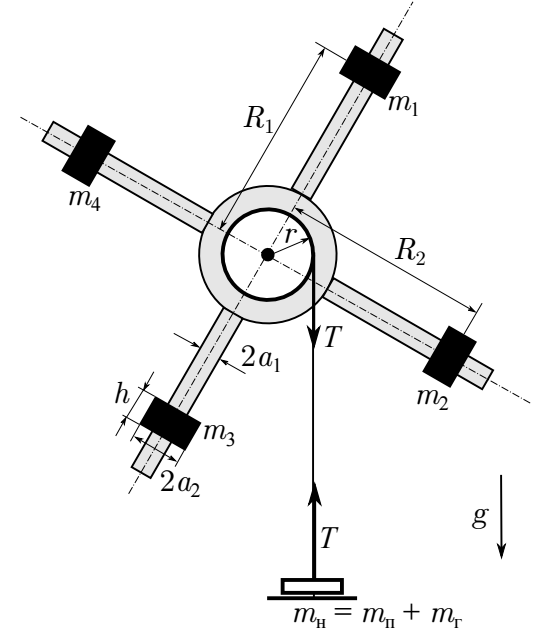
\includegraphics[width = 10cm]{Oberbek1}}
	\caption{Крестообразный маятник Обербека}
	\label{fig:image}
\end{figure}

Установка оснащена датчиком, позволяющим фиксировать моменты времени прохождения концов стержней через него. Данные с датчика передаются на компьютер для последующей обработки и получения зависимостей угла поворота $\varphi (t)$, угловой скорости $\omega = \varphi'$ и углового
ускорения маятника $\beta = \varphi''$ от времени, а также углового ускорения от угловой скорости $\beta(\omega)$.

\vspace{1cm}
\textbf{Вывод уравнения движения маятника.} Рассмотрим силы, действующие на маятник. Основной вращающий момент создаётся подвешенным на нити перегрузком. Непосредственно на маятник действует момент силы натяжения нити: $M_\text{н} = rT$, где $r$ --- радиус шкива ($r_1$ или $r_2$). Силу $T$ выразим из уравнения движения платформы: $m_\text{н}y'' = m_\text{н}g - T$, где $m_\text{н} = m_\text{п} + m_\text{г}$ --- масса платформы с перегрузком. Ускорение платформы связано с угловым ускорением маятника условием нерастяжимости нити $y'' = \beta r$. Отсюда момент силы натяжения нити

\begin{equation}
M_\text{н} = m_\text{н}r(g - \beta r)
\end{equation}

Вращению маятника препятствует момент силы трения в оси $M_\text{тр}$. Таким образом, с учетом (2) уравнение (1) может быть записано как

\begin{equation}
(I + m_\text{Н}r^2)\beta = m_\text{н}gr - M_\text{тр}
\end{equation}

Заметим, что в наших опытах, как правило, $m_\text{н}r^2 \ll 𝐼$, и соответственно, $M_\text{н} \approx m_\text{н}gr$. Если трение мало, $M_\text{тр} \ll m_\text{н}gr$, то маятник будет раскручиваться с постоянным угловым ускорением $\beta_0 \approx m_\text{н}gr/I$.

Поскольку зависимость момента силы трения от нагрузки на маятник и скорости его вращения не известна (её исследование --- отдельная экспериментальная задача), методика измерения должна быть построена так, чтобы минимизировать или вовсе исключить влияние $M_\text{тр}$. Можно высказать следующие качественные соображения о природе и величине $M_\text{тр}$. Она может иметь как составляющую, пропорциональную силе реакции в оси $N$ (сухое трение в подшипниках), так и составляющую, пропорциональную угловой скорости $\omega$ вращения маятника (вязкое трение в подшипниках и сопротивление воздуха). Учитывая, что сила реакции уравновешеннего маятника равна 
$N = m_\text{м}g + T \approx (m_\text{м} + m_\text{н})g \approx m_\text{м}g$, где $m_\text{м}$ — масса маятника (как правило, 
$M_\text{м} \gg m_\text{н}$), можно записать

\begin{equation}
M_\text{тр} \approx \left(1 + \frac{m_\text{н}}{m_\text{м}}\right)M_0 + \alpha\omega
\end{equation}

где $M_0$ --- момент сил трения для покоящегося маятника при нулевой массе подвеса (минимальное значение силы трения), $\alpha$ — некоторый
коэффициент, отвечающий за вязкое трение.

\vspace{1cm}
\textbf{Методика эксперимента.} Малость величины трения $M_\text{тр}$ в работе обеспечивается за счёт использования в креплении подшипников качения. Однако учёт трения всё же оказывается необходим, поскольку оно существенно влияет на результаты опыта как при малых массах перегрузков (когда $m_\text{н} \sim M_0/gr$), так и при больших, поскольку при увеличении $m_\text{н}$ возрастает сила реакции в оси и угловая скорость вращения маятника, а с ней и вязкое трение.

Влияние вязкой составляющей трения можно исключить следующим образом. Экспериментальная установка позволяет измерять зависимость углового ускорения от угловой скорости $\beta(\omega)$. Если верны высказанные выше соображения о величине силы трения, из (3) и (4) следует, что угловое ускорение должно быть линейной функцией угловой скорости: $\beta(\omega) = \beta_0 + k\omega$. В таком случае, определив по экспериментальным данным (с помощью расчётной программы) коэффициенты прямой, можно найти начальное угловое ускорение $\beta_0$, значение
которого и используется при проверке основного соотношения (3) при различных параметрах системы $(m_\text{н} , 𝐼 , 𝑟)$.

\vspace{1cm}
Проведем следующие измерения.

\vspace{0.5cm}
1. Исследуем вращательное движение маятника под действием различных перегрузков при постоянном моменте инерции системы $I$ (положения $R_i$ грузов фиксированы). Результатом будет зависимость начального углового ускорения $\beta_0$ от нагрузки $m_\text{н}$, откуда, согласно
(3), может быть определён момент инерции системы $I$ и минимальный момент силы трения $M_0$.

2. Затем изучим вращательное движение маятника при различных значениях момента инерции системы (фиксирована масса $m_\text{н}$). Момент инерции можно варьировать, изменяя расстояния $R_i$ центров масс грузов от оси вращения. Измеренные значения $I$ сравниваются с расчетными. Для расчётов воспользуемся тем,что грузы $m_i$ имеют форму полых цилиндров с внутренним и внешним радиусами $a_1$ и $a_2$ соответственно и образующей $h$, так что момент инерции всей системы вычисляется по теореме Гюйгенса–Штейнера:

\begin{equation}
I = I_0 + \sum_{i = 1}^4(I_i + m_iR_i^2)
\end{equation}

где $I_0$ – момент инерции системы без грузов,

\begin{equation}
I_i = \frac{1}{12}m_ih^2 + \frac{1}{4}m_i(a_1^2 + a_2^2)
\end{equation}

момент инерции $i$-го груза относительно оси, проходящей через его центр масс (перпендикулярно плоскости рис. 1). 

\vspace{1cm}
\textbf{Балансировка маятника.}
Для применимости соотношений (2)---(4) необходимо, чтобы маятник был уравновешен, то есть его центр масс должен находиться строго на оси вращения. Несбалансирован ность приводит к следующим эффектам: во-первых, появляется зависимость момента силы тяжести от угла поворота маятника; во-вторых, возникают дополнительные пульсации силы реакции $N$ (из-за центростремительного ускорения центра масс) и, следовательно, момента силы трения в подшипниках $M_\text{тр}$. Оба фактора могут привести к существенному отклонению от линейной зависимости измеряемой функции $\beta(\omega)$ (рис. 2). Слишком грубая балансировка делает формулы (2)---(4) полностью неприменимыми.

\begin{figure}[h!]
	\center{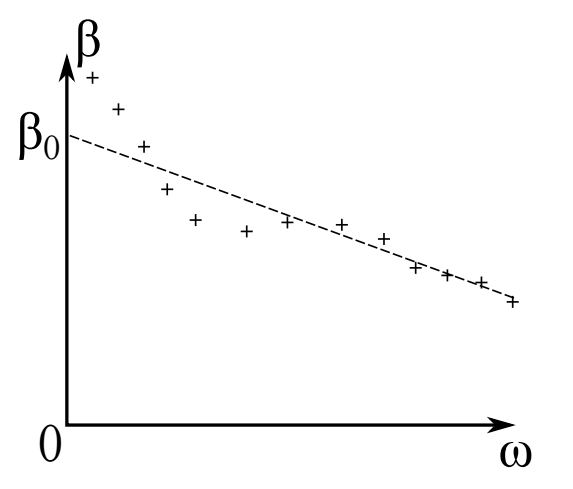
\includegraphics[width = 9cm]{Plot1}}
	\caption{Пульсации при вращении несбалансированного матяника}
	\label{fig:image}
\end{figure} 

Таким образом, для корректного проведения опыта необходима тщательная балансировка маятника при любом изменении положений грузов $m_i$ на стержнях. Маятник является сбалансированным, если он находится в безразличном положении равновесия. Для проверки балансировки необходимо привести маятник без подвеса во вращение с небольшой угловой скоростью, дав ему возможность остановиться. Если движение маятника не имеет колебательного характера (является апериодическим), систему можно считать сбалансированной. Кроме того, при быстром вращении несбалансированность маятника может быть определена по стуку в оси крепления.

\vspace{1cm}
\textbf{Ход работы.}

\vspace{1cm}
1. Установиv грузы $m_i$ на некотором (среднем) расстоянии $R$ от оси шкива так, чтобы маятник оказался в положении безразличного равновесия. Тщательно проведите балансировку, незначительно изменяя положения грузов. Платформа для подвешивания перегрузков должна при балансировке убирается. После балансировки измерим положения каждого груза $R_i$.

2. Оценим момент силы трения покоя $M_0$ в подшипниках. Для этого намотаем на меньший из шкивов нить в один слой и подвесим на ней к маятнику пустую платформу. Аккуратно нагрузим платформу так, чтобы маятник пришел в движение и запишем граничное значение $M_0$. Повторим измерение при других углах поворота маятника. Если маятник начинает совершать колебательные движения или необходимая для приведения маятника в движение масса зависит от угла поворота маятника, еще раз уточним балансировку. Если маятник приходит во вращение без перегрузков, значит момент
сил мал, $M_0 < m_\text{п}gr$, и таким методом его измерить невозможно.

3. Включим компьютер и запустим программу "Kinematic". Ознакомьтесь с краткой инструкцией по работе с программой (см. Приложение). При необходимости обратитесь к полной инструкции (на столах) или справке внутри программы.

4. Намотайте нить в один слой на больший из шкивов и поместите перегрузок ($m_\text{н} \sim$ г) на платформу. Проведите опыт: с помощью программы измерьте зависимость угла поворота маятника от времени в процессе опускания платформы из верхнего в нижнее положение.

По завершении опыта перейдите в раздел "Определение углового ускорения". На экране будет представлен график зависимости углового ускорения от угловой скорости $\beta(\omega)$. Программа проводит через экспериментальные точки прямую методом наименьших квадратов (МНК). Запишите полученные коэффициенты $\beta_0$ и $k$ прямой $\beta = \beta_0 + k\omega$ и их погрешности (рассчитанные также по МНК).

При необходимости программа позволяет провести отбор экспериментальных точек, которые используются для проведения прямой. Из рассмотрения можно исключить несколько начальных точек (поскольку для них существенно влияние силы трения покоя), а также, возможно, конечные точки, соответствующие изменению направления движения платформы. При наличии резких выбросов (ошибки срабатывания датчика) опыт переделаем. Если на полученном графике существенны колебания зависимости $\beta(\omega)$ относительно прямой, уточните балансировку и повторите измерение. Если дальнейшее уточнение балансировки затруднено, грубо оценим погрешность, вносимую этими колебаниями в результат опыта. 

5. Для оценки случайной погрешности опыта проведем 6---8 измерений по п. 4 для фиксированных значений массы и момента инерции маятника. По результатам оцените случайную ошибку $\sigma_{\beta}$.

6. Проведем опыт п. 4. для 6---8 значений момента силы натяжения нити, используя перегрузки $m_\text{г}$ в диапазоне от 20 до 200 г на разных
шкивах.

7. Измерим зависимость углового ускорения от момента инерции системы. Для этого при одном из значений массы перегрузка из предыдущего пункта ($m_\text{г} \sim 200$г) проведем измерения $\beta_0$ и $k$ при 4---5 различных значениях расстояния $R$ от оси системы до центров масс грузов. После перемещения грузов заново проводим балансировку балансировку.

8. Снимем грузы со стержней и проведем несколько опытов по опусканию грузов для определения момента инерции пустой конструкции $I_0$.

9. По результатам п. 6 проверим справедливость формулы (3). Для этого построим график зависимости начального углового ускорения $\beta_0(M_\text{н})$ от момента силы натяжения нити (2). Убедимся, что экспериментальные точки ложатся на прямую линию. По наклону прямой определим момент инерции $I$, а по пересечению с осью абсцисс --- минимальную силу трения $M_0$. Сравним $M_0$ с измеренным в п. 2. Оценим погрешности результатов.

10. Пользуясь формулой (3) и величиной $M_0$, полученной в п. 9, рассчитаем по результатам п. 7 моменты инерции $I$ системы при различных $R$. Оценим погрешность измерения $I$. Построим график зависимости $I(R^2)$. Используя график и формулы (5)–(6), определим момент инерции конструкции без грузов $I_0$ и сравним его с измеренным в п. 8.

\vspace{1cm}
Измерения.

\vspace{1cm}
Найдем $M_0$. Маятник начинает движение, если положить грузик массой $m_0 = 3.6$г, то есть $M_0 = 1.8 \cdot 10^{-3} H\cdot\text{м}$.

\vspace{1cm}

Масса подвеса $m_\text{п} = 15.7$г. 
Массы грузиков и их расстояния до оси:
\begin{center}
\begin{tabular}{|l|c|c|c|c|c|c|c|c|}
\hline
Номер грузика			&	1		&	2		&	3		&	4		\\
\hline
Масса грузика, г		&	155.5	&	148.9	&	151.9	&	150.1	\\
\hline
Расстояние до оси, cм	&	6.7		&	7.4		&	6.5		&	7.1		\\
\hline
\end{tabular}
\end{center}

Измерения:
\begin{center}
\begin{tabular}{|c|c|c|c|c|c|c|c|c|c|c|c|c|c|c|c|}
\hline
$m_\text{г}$,г	&\multicolumn{4}{|c|}{50 г}			\\
\hline
$m_\text{н}$,г	&\multicolumn{4}{|c|}{65 г}		\\
\hline
				&	$\beta$, рад/$c^2$		&	$k$, 1/c		&	$\delta\beta$, рад/$c^2$		&	$\delta k$, 1/c			\\
\hline
				&	0.661					&	-0.016			&	0.003							&	0.006					\\
\hline
				&	0.660					&	-0.017			&	0.003							&	0.007					\\
\hline
				&	0.665					&	-0.014			&	0.004							&	0.006					\\
\hline
				&	0.657					&	-0.015			&	0.003							&	0.005					\\
\hline
				&	0.668					&	-0.018			&	0.002							&	0.007					\\
\hline
				&	0.661					&	-0.016			&	0.003							&	0.006					\\
\hline
\end{tabular}
\end{center}

\begin{center}
\begin{tabular}{|c|c|c|c|c|c|c|c|c|c|c|c|c|c|c|c|}
\hline
$m_\text{г}$,г	&\multicolumn{4}{|c|}{100 г}		\\
\hline
$m_\text{н}$,г	&\multicolumn{4}{|c|}{115 г}		\\
\hline
				&	$\beta$, рад/$c^2$		&	$k$, 1/c		&	$\delta\beta$, рад/$c^2$		&	$\delta k$, 1/c			\\
\hline
				&	1.188					&	-0.017			&	0.003							&	0.002					\\
\hline
				&	1.191					&	-0.016			&	0.004							&	0.002					\\
\hline
				&	1.194					&	-0.015			&	0.004							&	0.004					\\
\hline
				&	1.186					&	-0.017			&	0.003							&	0.003					\\
\hline
				&	1.189					&	-0.018			&	0.004							&	0.004					\\
\hline
				&	1.189					&	-0.016			&	0.004							&	0.003					\\
\hline
\end{tabular}
\end{center}

\begin{center}
\begin{tabular}{|c|c|c|c|c|c|c|c|c|c|c|c|c|c|c|c|}
\hline
$m_\text{г}$,г	&\multicolumn{4}{|c|}{150 г}			\\
\hline
$m_\text{н}$,г	&\multicolumn{4}{|c|}{165 г}		\\
\hline
				&	$\beta$, рад/$c^2$		&	$k$, 1/c		&	$\delta\beta$, рад/$c^2$		&	$\delta k$, 1/c			\\
\hline
				&	1.820					&	-0.018			&	0.005							&	0.002					\\
\hline
				&	1.823					&	-0.018			&	0.006							&	0.003					\\
\hline
				&	1.831					&	-0.017			&	0.005							&	0.004					\\
\hline
				&	1.825					&	-0.019			&	0.004							&	0.005					\\
\hline
				&	1.827					&	-0.018			&	0.006							&	0.003					\\
\hline
				&	1.826					&	-0.018			&	0.005							&	0.004					\\
\hline
\end{tabular}
\end{center}

\begin{center}
\begin{tabular}{|c|c|c|c|c|c|c|c|c|c|c|c|c|c|c|c|}
\hline
$m_\text{г}$,г	&\multicolumn{4}{|c|}{200 г}			\\
\hline
$m_\text{н}$,г	&\multicolumn{4}{|c|}{215 г}		\\
\hline
				&	$\beta$, рад/$c^2$		&	$k$, 1/c		&	$\delta\beta$, рад/$c^2$		&	$\delta k$, 1/c			\\
\hline
				&	2.381					&	-0.020			&	0.005							&	0.003					\\
\hline
				&	2.383					&	-0.023			&	0.004							&	0.004					\\
\hline
				&	2.385					&	-0.022			&	0.006							&	0.005					\\
\hline
				&	2.376					&	-0.019			&	0.004							&	0.004					\\
\hline
				&	2.379					&	-0.017			&	0.004							&	0.003					\\
\hline
				&	2.382					&	-0.020			&	0.004							&	0.004					\\
\hline
\end{tabular}
\end{center}

\begin{center}
\begin{tabular}{|c|c|c|c|c|c|c|c|c|c|c|c|c|c|c|c|}
\hline
$m_\text{г}$,г	&\multicolumn{4}{|c|}{130}			\\
\hline
$m_\text{н}$,г	&\multicolumn{4}{|c|}{145}		\\
\hline
				&	$\beta$, рад/$c^2$		&	$k$, 1/c		&	$\delta\beta$, рад/$c^2$		&	$\delta k$, 1/c			\\
\hline
				&	1.589					&	0.017			&	0.004							&	0.004					\\
\hline
				&	1.590					&	0.019			&	0.004							&	0.004					\\
\hline
				&	1.595					&	0.018			&	0.005							&	0.003					\\
\hline
				&	1.585					&	0.017			&	0.003							&	0.005					\\
\hline
				&	1.594					&	0.016			&	0.004							&	0.004					\\
\hline
				&	1.593					&	0.017			&	0.004							&	0.004					\\
\hline
\end{tabular}
\end{center}

\begin{center}
\begin{tabular}{|c|c|c|c|c|c|c|c|c|c|c|c|c|c|c|c|}
\hline
$m_\text{г}$,г	&\multicolumn{4}{|c|}{170}			\\
\hline
$m_\text{н}$,г	&\multicolumn{4}{|c|}{185}		\\
\hline
				&	$\beta$, рад/$c^2$		&	$k$, 1/c		&	$\delta\beta$, рад/$c^2$		&	$\delta k$, 1/c			\\
\hline
				&	2.055					&	0.019			&	0.005							&	0.003					\\
\hline
				&	2.049					&	0.016			&	0.003							&	0.003					\\
\hline
				&	2.050					&	0.020			&	0.006							&	0.004					\\
\hline
				&	2.052					&	0.018			&	0.006							&	0.002					\\
\hline
				&	2.053					&	0.019			&	0.003							&	0.006					\\
\hline
				&	2.053					&	0.019			&	0.005							&	0.004					\\
\hline
\end{tabular}
\end{center}

\vspace{1cm}
Построим график $\beta_0(m_\text{н})$:

\vspace{1cm}
\begin{flushleft}
\begin{tikzpicture}
\begin{axis}[
	height = 9cm,
	width  = 14cm,
	every axis y label/.style={at = {(ticklabel cs: 0.5)}, rotate = 90, anchor = near ticklabel},
	xlabel = {$m_\text{н}, g$},
	ylabel = {$\beta, rad/sec^2$}
]
\addplot+[error bars/.cd, 
	y dir = both, y explicit,
	x dir = both, x explicit,
	]
coordinates{
	%(0,0)
	( 65, 0.661) +- (0, 0.003)
	(115, 1.198) +- (0, 0.004)
	(145, 1.593) +- (0, 0.005) 
	(165, 1.826) +- (0, 0.004)
	(185, 2.052) +- (0, 0.005)
	(215, 2.382) +- (0, 0.005)
};
\end{axis}
\end{tikzpicture}
\end{flushleft}

\vspace{1cm}
График линеен. По нему определим значения $I$ и $M_0$:
%min = 87
%max = 92
$$I = (7.9 \pm 0.2) \cdot 10^{-3} \text{кг}\cdot\text{м}^2$$
%min = 6
%max = 20
$$M_0 = (1.2 \pm 0.6)\cdot 10^{-3} \text{Н}\cdot\text{м}$$

Видно, что полученное значение близко к измеренному напрямую.	

\vspace{1cm}
Используем перегрузок 100г.

% I = (M - M_0)/b

\begin{center}
\begin{tabular}{|c|c|c|c|c|c|c|c|c|c|c|c|c|c|c|c|}
\hline
$R$,см	&	\multicolumn{5}{|c|}{6}			\\
\hline
$R^2, \text{см}^2$	&	\multicolumn{5}{|c|}{36}			\\
\hline
		&	$\beta$, рад/$c^2$	&	$k$, 1/c	&	$\delta\beta$, рад/$c^2$	&	$\delta k$, 1/c		&	$I$		\\
\hline
		&	2.422				&	-0.031		&	0.008						&	0.003				&	0.0037	\\
\hline
		&	2.426				&	-0.030		&	0.007						&	0.003				&	0.0036	\\
\hline
		&	2.420				&	-0.028		&	0.007						&	0.002				&	0.0037	\\
\hline
		&	2.425				&	-0.032		&	0.009						&	0.004				&	0.0036	\\
\hline
		&	2.423				&	-0.030		&	0.008						&	0.003				&	0.0037	\\
\hline
\end{tabular}
\end{center}

\begin{center}
\begin{tabular}{|c|c|c|c|c|c|c|c|c|c|c|c|c|c|c|c|}
\hline
$R$,см	&	\multicolumn{5}{|c|}{9}			\\
\hline
$R^2, \text{см}^2$	&	\multicolumn{5}{|c|}{81}			\\
\hline
		&	$\beta$, рад/$c^2$	&	$k$, 1/c	&	$\delta\beta$, рад/$c^2$	&	$\delta k$, 1/c		&	$I$		\\
\hline
		&	1.826				&	-0.023		&	0.006						&	0.002				&	0.0049	\\
\hline
		&	1.823				&	-0.022		&	0.004						&	0.003				&	0.0050	\\
\hline
		&	1.824				&	-0.020		&	0.004						&	0.002				&	0.0049	\\
\hline
		&	1.830				&	-0.021		&	0.004						&	0.003				&	0.0049	\\
\hline
		&	1.826				&	-0.022		&	0.005						&	0.002				&	0.0049	\\
\hline
\end{tabular}
\end{center}

\begin{center}
\begin{tabular}{|c|c|c|c|c|c|c|c|c|c|c|c|c|c|c|c|}
\hline
$R$,см	&	\multicolumn{5}{|c|}{12}			\\
\hline
$R^2, \text{см}^2$	&	\multicolumn{5}{|c|}{144}			\\
\hline
		&	$\beta$, рад/$c^2$	&	$k$, 1/c	&	$\delta\beta$, рад/$c^2$	&	$\delta k$, 1/c		&	$I$		\\
\hline
		&	1.364				&	-0.018		&	0.006						&	0.002				&	0.0066	\\
\hline
		&	1.364				&	-0.017		&	0.004						&	0.003				&	0.0066	\\
\hline
		&	1.366				&	-0.016		&	0.003						&	0.002				&	0.0065	\\
\hline
		&	1.365				&	-0.017		&	0.005						&	0.002				&	0.0066	\\
\hline
		&	1.364				&	-0.017		&	0.004						&	0.002				&	0.0066	\\
\hline
\end{tabular}
\end{center}

\begin{center}
\begin{tabular}{|c|c|c|c|c|c|c|c|c|c|c|c|c|c|c|c|}
\hline
$R$,см	&	\multicolumn{5}{|c|}{15}			\\
\hline
$R^2, \text{см}^2$	&	\multicolumn{5}{|c|}{225}			\\
\hline
		&	$\beta$, рад/$c^2$	&	$k$, 1/c	&	$\delta\beta$, рад/$c^2$	&	$\delta k$, 1/c		&	$I$		\\
\hline
		&	1.034				&	-0.015		&	0.006						&	0.004				&	0.0087	\\
\hline
		&	1.030				&	-0.013		&	0.004						&	0.003				&	0.0088	\\
\hline
		&	1.035				&	-0.016		&	0.004						&	0.004				&	0.0087	\\
\hline
		&	1.034				&	-0.013		&	0.004						&	0.003				&	0.0087	\\
\hline
		&	1.034				&	-0.014		&	0.005						&	0.004				&	0.0087	\\
\hline
\end{tabular}
\end{center}

\begin{center}
\begin{tabular}{|c|c|c|c|c|c|c|c|c|c|c|c|c|c|c|c|}
\hline
$R$,см	&	\multicolumn{5}{|c|}{18}			\\
\hline
$R^2, \text{см}^2$	&	\multicolumn{5}{|c|}{324}			\\
\hline
		&	$\beta$, рад/$c^2$	&	$k$, 1/c	&	$\delta\beta$, рад/$c^2$	&	$\delta k$, 1/c		&	$I$		\\
\hline
		&	0.803				&	-0.011		&	0.004						&	0.002				&	0.0112	\\
\hline
		&	0.800				&	-0.010		&	0.004						&	0.004				&	0.0112	\\
\hline
		&	0.799				&	-0.009		&	0.003						&	0.003				&	0.0113	\\
\hline
		&	0.805				&	-0.010		&	0.003						&	0.003				&	0.0012	\\
\hline
		&	0.803				&	-0.010		&	0.003						&	0.003				&	0.0012	\\
\hline
\end{tabular}
\end{center}

\begin{center}
\begin{tabular}{|c|c|c|c|c|c|c|c|c|c|c|c|c|c|c|c|}
\hline
$R$,см	&	\multicolumn{5}{|c|}{0}			\\
\hline
$R^2, \text{см}^2$	&	\multicolumn{5}{|c|}{0}			\\
\hline
		&	$\beta$, рад/$c^2$	&	$k$, 1/c	&	$\delta\beta$, рад/$c^2$	&	$\delta k$, 1/c		&	$I$		\\
\hline
		&	3.440				&	-0.007		&	0.002						&	0.005				&	0.027	\\
\hline
		&	3.443				&	-0.009		&	0.004						&	0.004				&	0.027	\\
\hline
		&	3.441				&	-0.008		&	0.003						&	0.006				&	0.027	\\
\hline
		&	3.444				&	-0.008		&	0.003						&	0.003				&	0.026	\\
\hline
		&	3.443				&	-0.008		&	0.003						&	0.004				&	0.027	\\
\hline
\end{tabular}
\end{center}

\vspace{1cm}
\begin{flushleft}
\begin{tikzpicture}
\begin{axis}[
	height = 9cm,
	width  = 14cm,
	every axis y label/.style={at = {(ticklabel cs: 0.5)}, rotate = 90, anchor = near ticklabel},
	xlabel = {$R^2, \text{cm}^2$},
	ylabel = {$I, kg \cdot m^2$}
]
\addplot+[error bars/.cd, 
	y dir = both, y explicit,
	x dir = both, x explicit,
	]
coordinates{
	%(0,0)
	( 36, 0.0037) +- (0, 0)
	( 81, 0.0049) +- (0, 0)
	(144, 0.0066) +- (0, 0) 
	(225, 0.0087) +- (0, 0)
	(324, 0.0112) +- (0, 0)
};
\end{axis}
\end{tikzpicture}
\end{flushleft}

%Из графика - 0.27 и 0.31
Продлив график до пересечения с осью $I$ при $m = 0$ определим $I_0$:

$$\boxed{I_0 = (2.9 \pm 0.2)\cdot 10^{-3}\text{кг}\cdot\text{м}^2}$$



\end{document}
